\documentclass[12pt, a4paper]{article}
\usepackage[utf8]{inputenc}
\usepackage{amsmath}
\usepackage{amsfonts}
\usepackage{amssymb}
\usepackage{graphicx}
\usepackage{caption}
\usepackage{subcaption}
\usepackage{sidecap}
\author{MORAES, FELIPE}
\title{Fundamentals of STDP based recurrent assembly networks}

\newtheorem{theorem}{Theorem}[section]
\newtheorem{lemma}[theorem]{Lemma}
\newtheorem{proposition}[theorem]{Proposition}
\newtheorem{corollary}[theorem]{Corollary}

\newenvironment{proof}[1][Proof]{\begin{trivlist}
\item[\hskip \labelsep {\bfseries #1}]}{\end{trivlist}}
\newenvironment{definition}[1][Definition]{\begin{trivlist}
\item[\hskip \labelsep {\bfseries #1}]}{\end{trivlist}}
\newenvironment{example}[1][Example]{\begin{trivlist}
\item[\hskip \labelsep {\bfseries #1}]}{\end{trivlist}}
\newenvironment{remark}[1][Remark]{\begin{trivlist}
\item[\hskip \labelsep {\bfseries #1}]}{\end{trivlist}}

\newcommand{\qed}{\nobreak \ifvmode \relax \else
      \ifdim\lastskip<1.5em \hskip-\lastskip
      \hskip1.5em plus0em minus0.5em \fi \nobreak
      \vrule height0.75em width0.5em depth0.25em\fi}

\renewcommand{\figurename}{Figura}

\begin{document}

\begin{center}
{\huge TRABALHO PRÁTICO 3: Expansor de Macros}

\textit{Felipe Moraes Gomes - felipemoraes@dcc.ufmg.br}
\end{center}

\section{Introdução e Definição do Trabalho}
Este trabalho descreve a implementação e operação de um expansor de macros para uma linguagem assembly hipotética, baseada no conjunto de instruções do RISC. O programa recebe como entrada um arquivo de texto, contendo código, e identifica as macros nele, efetuando sua expansão.

O restante deste documento está organizado da seguinte forma: A 2\textsuperscript{a} seção trata da implementação do expansor e de sua organização no código; A 3\textsuperscript{a} seção resume o formato de execução, entrada e saída do programa; A 4\textsuperscript{a} seção contém os testes realizados; A 5\textsuperscript{a} seção conclui o trabalho. Após isso, é colocado um apêndice contendo uma listagem dos arquivos do projeto. 

\section{Implementação e Organização}

O expansor abre o arquivo de código especificado e efetua sua expansão em dois passos. Na primeira leitura, todos os macros são identificados e armazenados. Em seguida, uma segunda leitura é realizada substituindo as macros identificadas por uma instanciação de seu código.

O código foi implementado através de funções e procedimentos com uma estrutura de dados para auxiliar o armazenado e expansão das macros, delimitadas a seguir.

\subsection{Dados e Variáveis}


\begin{itemize}
	\item \emph{vector{\tt<}struct{\tt>} Macro}: Armazena as macros obtidas no primeiro passo.	
	\item \emph{struct{\tt<}Macro{\tt>}}: Armazena o tipo de cada macro nos campos do registro. Os tipos são \emph{Label}, \emph{Parameter} (se for uma instancia do parâmetro da macro), e \emph{Body} (código identificado).
\end{itemize}

\subsection{Procedimentos e Funções}
\begin{itemize}
	\item \emph{int ExtractMacros(char* filename, Macros)}: Dado o nome do arquivo, extrai todas macros existente no programa de entrada e armazena em um conjunto de Macros retornando o número de macros encontradas. 
	\item \emph{void ExpandMacros(char* input, char* output, Macro* Macros, int num)}: Lê uma linha do arquivo de fonte, se for uma instrução imprime no arquivo de saida, se não procura pela macro preenchendo com parametros passados para ela.	
	\item \emph{char* SearchMacro(char *Label\_macro, Macro *Macros, char *Parameter, int num)}: Dado um label, procura uma macro no conjunto de Macros, caso a macro tenha um parametro a função \emph{ReplaceParameter} é chamada e em seguida a função retorna uma \emph{string} contendo o corpo da macro.
	\item \emph{char* ReplaceParameter(Macro macro, char *Parameter)}: Substitui na macro fornecida como entrada, o parâmetro, retornando uma \emph{string} contendo o corpo da macro.
\end{itemize}

\subsection{Fluxo de Execução}

O programa inicialmente lê os parâmetros passados a ele, verificando seu formato. Caso correto, ele chama \emph{ExpanderExpand}, que primeiro identifica as macros, e depois gera o arquivo de saída, em formato de código, já se tendo efetuado as expansões. Após retornar, o programa conclui sua execução.

\section{Controle \& IO}

\subsection{Execução e Compilação do Expansor}

O programa pode ser compilado através do g++, pelo utilitário \emph{make}, usando o makefile providenciado. Uma vez compilado, chamadas devem seguir o formato:

\begin{center}
\emph{./bin/expansor input.amk output.amk}
\end{center}

Onde \emph{input} e \emph{output} são os arquivos de código com e sem macros, respectivamente.

\subsection{Formato dos Arquivos de Entrada e Saída}

Cada linha dos programas em assembly devem seguir o formato:

\begin{center}
[{\tt<}label{\tt>}:] {\tt<}instrução{\tt>} {\tt<}operando1{\tt>} {\tt<}operando2{\tt>} [; comentário]
\end{center}

Onde \emph{label} e \emph{comentário} são opcionais, porém devendo ser devidamente delimitados (o sufixo ``:'' para o label e o prefixo ``;'' para o comentário). O tipo e quantidade dos operandos é dependente da instrução.

Macros são delimitados por \emph{BEGINMACRO} e \emph{ENDMACRO}, podendo haver um parâmetro opcional, permitindo substituição literal nas instanciações das macros. Não podem haver definições ou declarações de macros dentro de outras macros;

O arquivo de saída obtido obedece o mesmo formato do arquivo de entrada, excetuando a presença de macros, que sofreram substituição.

\section{Testes}

\begin{figure}
\centering
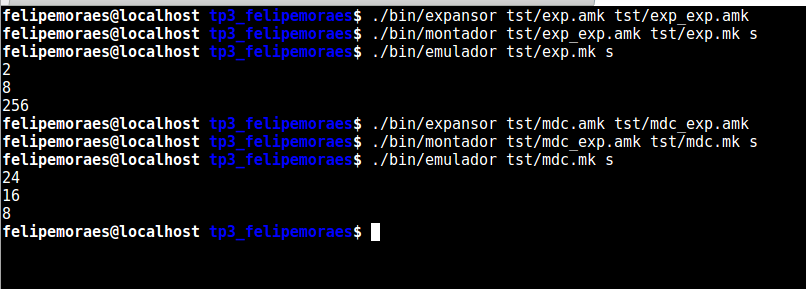
\includegraphics[width=1.0\textwidth]{RuntimeScreencap.png}
\caption{Compilação e execução dos testes}
\label{FigureExecution}
\end{figure}

Vários programas foram testados, de forma a obter cobertura total do código. Os testes podem ser executados na MV tornando \emph{PC = EndInicial = 0} e \emph{SP = 1000}. Os testes fizeram forte uso do expansor de macros, que promove grandes alterações sintáticas, visando aproximar uma linguagem mais alta.

\begin{itemize}
	\item \emph{Exponenciação (exp.amk):} Recebe dois parâmetros \emph{A} e \emph{B}, e imprime o resultado de $A^B$. Para tal, são computados os valores de $A^{2^i}$ onde $i \in (1, 32)$, que, subsequentemente, são multiplicados uns com os outros até que a soma dos expoente dê $B$. O algoritmo é $O(log(B) log(A))$, pois cada produto é $O(log(A))$ e o número de produtos é $O(log(B))$.
	\item \emph{MDC (mdc.amk):} Recebe dois números, e imprime o máximo divisor comum (MDC) deles. O cálculo é feito usando o algoritmo de MCD binário (uma extensão do algoritmo Euclidiano), e é $O(log^2(AB))$.
\end{itemize}

\section{Conclusão}

O expansor é eficaz em lidar com programas que fazem uso extensivo de macros, permitindo a construção de estruturas que auxiliem na elevação no nível da linguagem.

A execução do trabalho transcorreu sem maiores dificuldades, e os resultados obtidos correspondem ao esperado.

\appendix
\section{Apêndice}
\subsection{Listagem de Arquivos}
\begin{itemize}
	\item Código Fonte:
	\begin{itemize}
		\item \emph{src/main.c:} Interpreta os parâmetros de entrada e controla o fluxo do programa (Seção 2.3).
		\item \emph{src/expander.c, src/expander.h:} Implementa o expansor (Seção 2.2).
		\item \emph{src/io.c, src/io.h:} Implementa instruções de entrada e saida.
		\item \emph{src/Makefile:} Makefile para facilitar a compilação do programa (Seção 3.1).
	\end{itemize}
	\item Testes:
	Para cada teste, existe um \emph{.sbasm} (o programa com macros), um \emph{.sbint} (o código intermediário, sem macros) e um \emph{.sbexe} (o executável que roda na MV).
	\begin{itemize}
		\item \emph{tst/exp.amk}: (Seção 4 item 1).
		\item \emph{tst/mdc.amk}: (Seção 4 item 2).
	\end{itemize}
	
\end{itemize}

\end{document}
